\newpage
\section{Kết quả triển khai và đánh giá}

\subsection*{Triển khai}

Giao diện \textit{hệ thống quản lý} được xây dựng với thư viện \href{https://reactjs.org}{\textit{React}} (được phát triển bởi đội ngũ \textit{Facebook} với sự đóng góp của cộng đồng) sử dụng ngôn ngữ lập trình \href{https://www.typescriptlang.org/}{\textit{TypeScript}}. Đồng thời, người dùng cần đồng ý kết nối ví mã hoá \textit{MetaMask} với hệ thống để sử dụng các tính năng tương tác với hợp đồng thông minh. Phía máy chủ, \href{https://nodejs.org}{\textit{Node.js}} được lựa chọn, ta sử dụng \href{https://expressjs.com/}{\textit{Express}} để tạo các \textit{API}\footnote{Application Programming Interface}. Thông tin cần thiết được lấy từ cơ sở dữ liệu, và việc trao đổi giữa máy chủ và giao diện được thực hiện qua kết nối \textit{HTTP} và \textit{Web Socket}, các cập nhật từ một người sẽ được thông báo ngay lập tức tới các cá nhân khác trong cùng cơ sở cấp phát văn bằng.\\

\textit{Hệ thống tra cứu} sử dụng cấu trúc \textit{trang tĩnh}\footnote{Static web}, triển khai trên \textit{GitHub Pages} với mã nguồn công khai, cung cấp cho người dùng một công cụ tra cứu thông tin văn bằng nhanh chóng, đáng tin cậy. Các doanh nghiệp có thể lấy danh sách \textit{địa chỉ ví} của các cơ sở giáo dục tại trang thông tin (website) của cơ sở giáo dục đó, hoặc lấy từ một cơ quan có độ tin cậy lớn (như \textit{Bộ Giáo dục và Đào tạo} chẳng hạn). Thông tin số hiệu văn bằng sẽ được ứng viên cung cấp.\\

Dưới đây là một số hình ảnh khi người dùng trải nghiệm hệ thống, và em xin lưu ý \textit{đây chưa phải là hình ảnh của hệ thống hoàn thiện}.\\

\newpage
\begin{figure}[!ht]
    \centering
    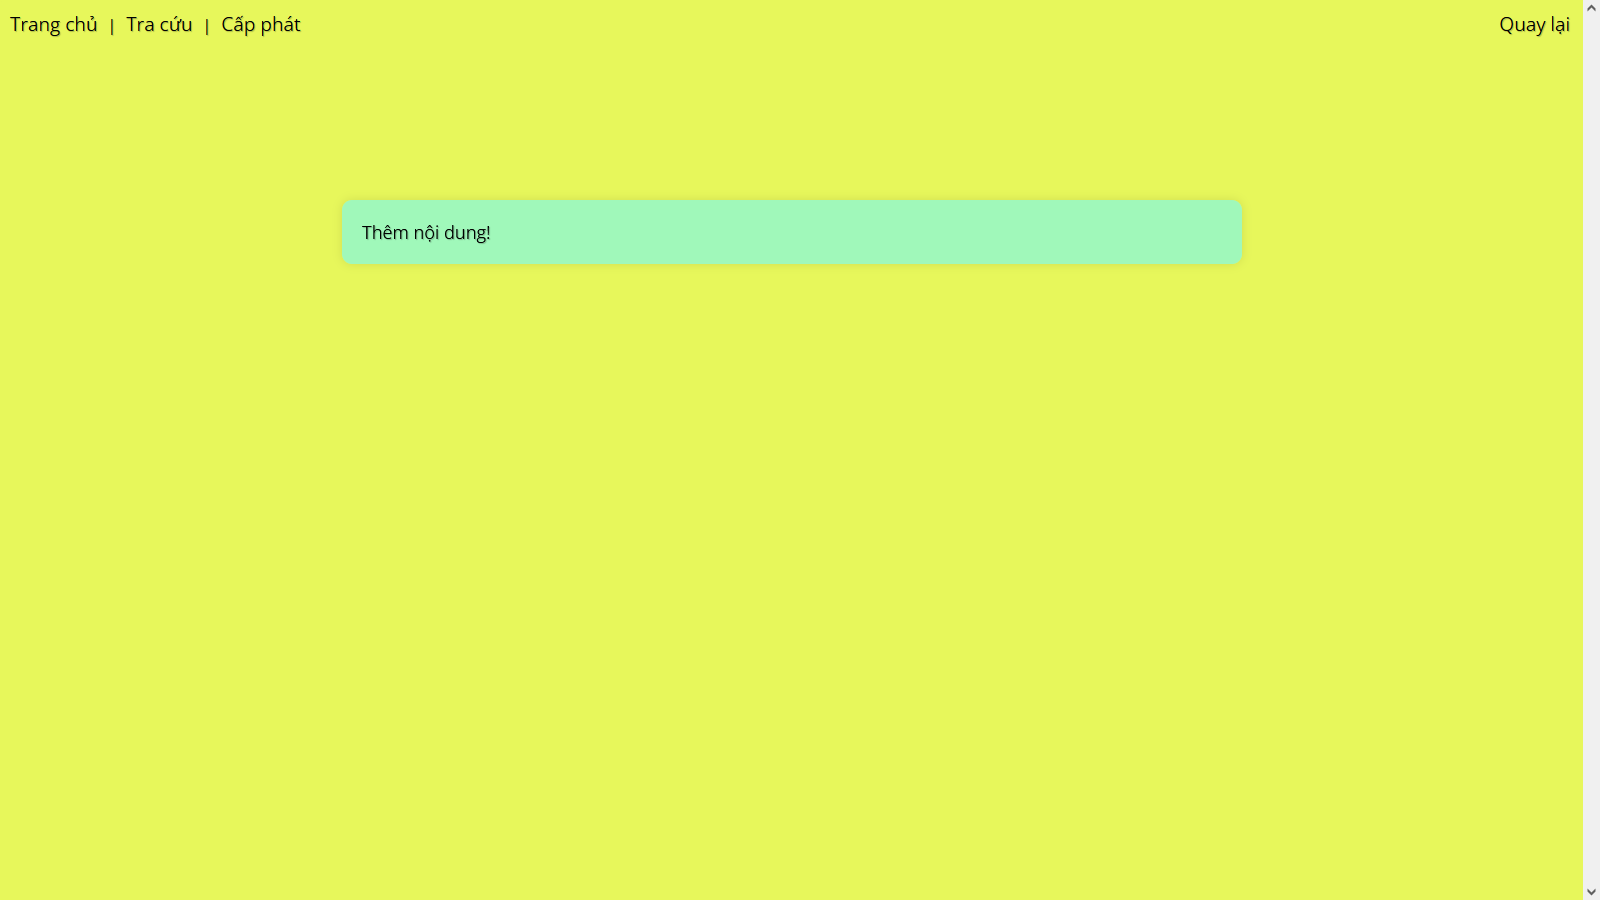
\includegraphics[width=350px]{anh/giai-phap/giao-dien-cap-phat-1.png}
    \caption{Một phần giao diện cấp phát văn bằng (1)}
\end{figure}
\begin{figure}[!ht]
    \centering
    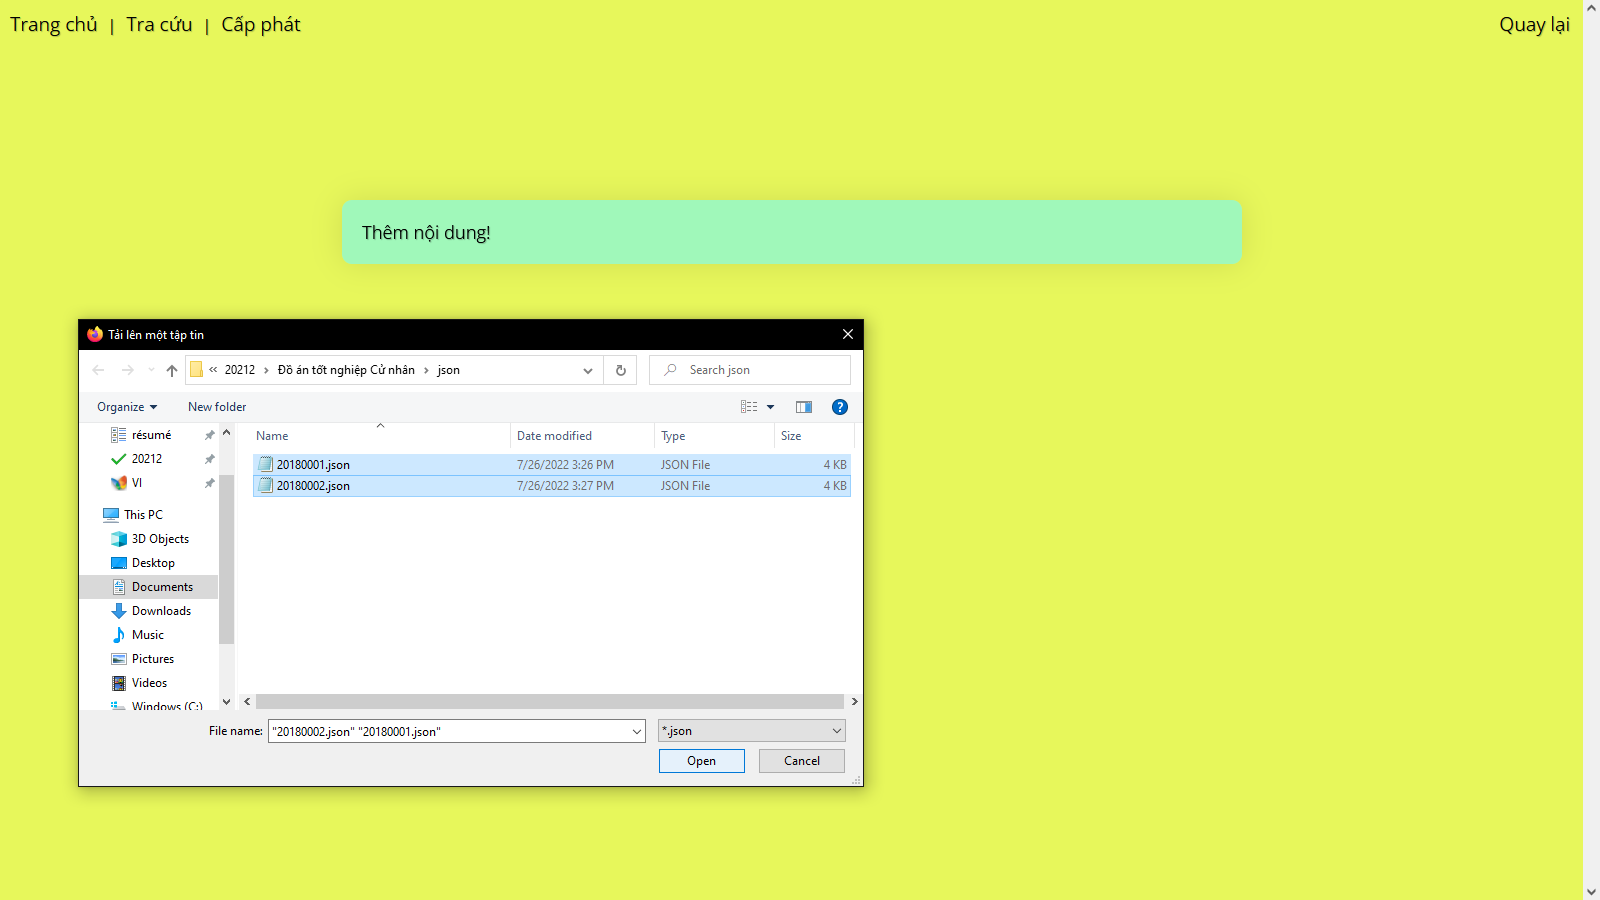
\includegraphics[width=350px]{anh/giai-phap/giao-dien-cap-phat-2.png}
    \caption{Một phần giao diện cấp phát văn bằng (2)}
\end{figure}

\newpage
\begin{figure}[!ht]
    \centering
    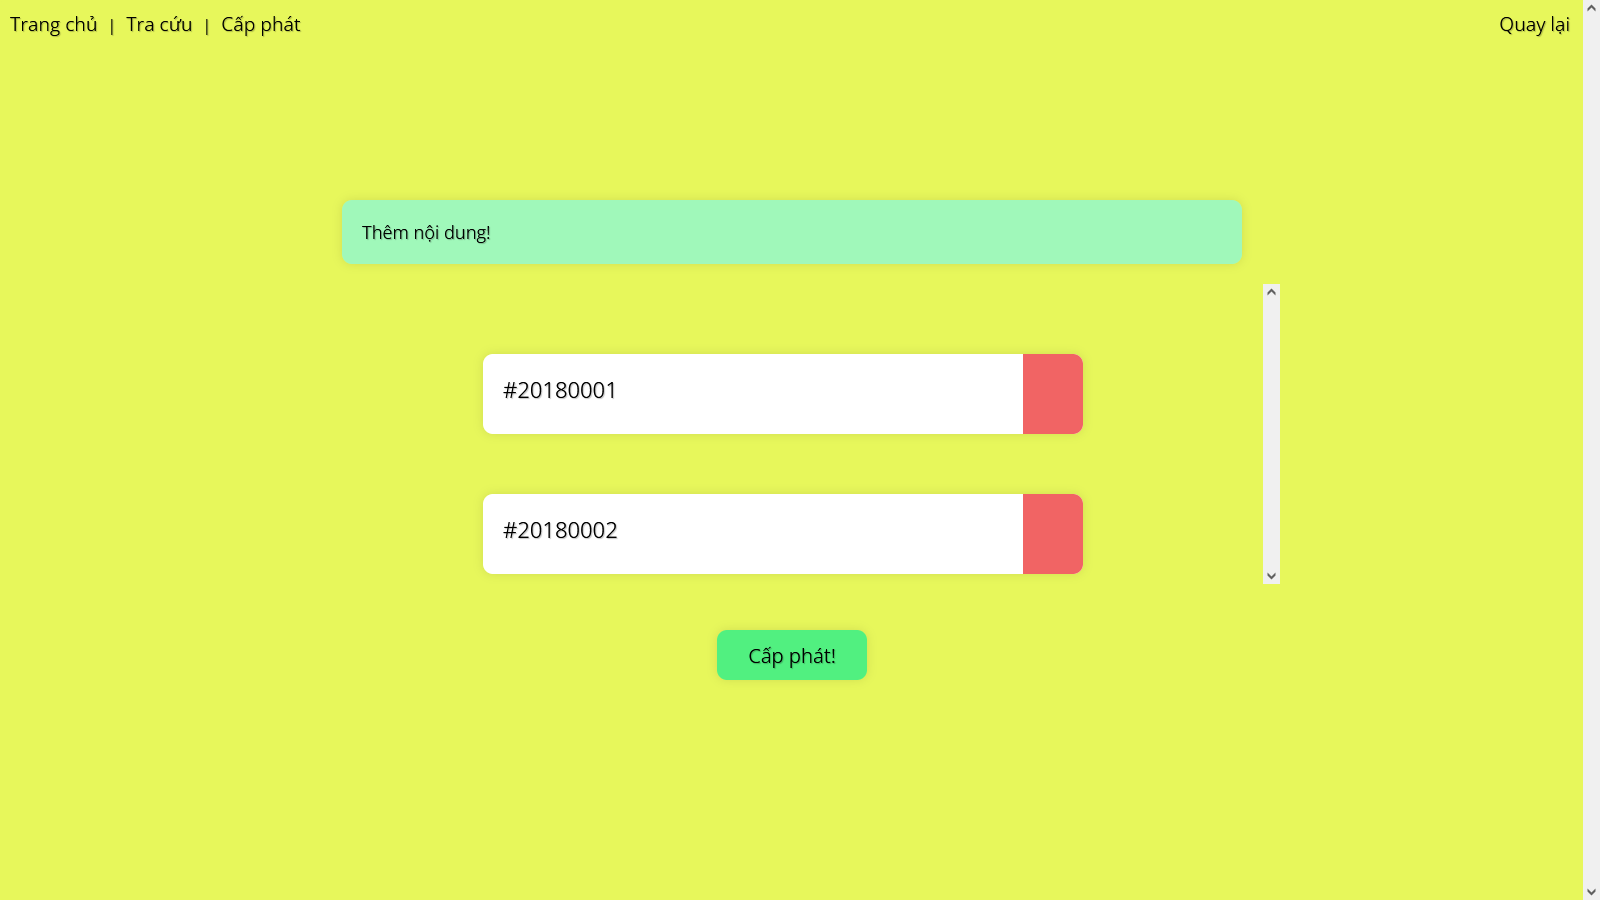
\includegraphics[width=350px]{anh/giai-phap/giao-dien-cap-phat-3.png}
    \caption{Một phần giao diện cấp phát văn bằng (3)}
\end{figure}
\begin{figure}[!ht]
    \centering
    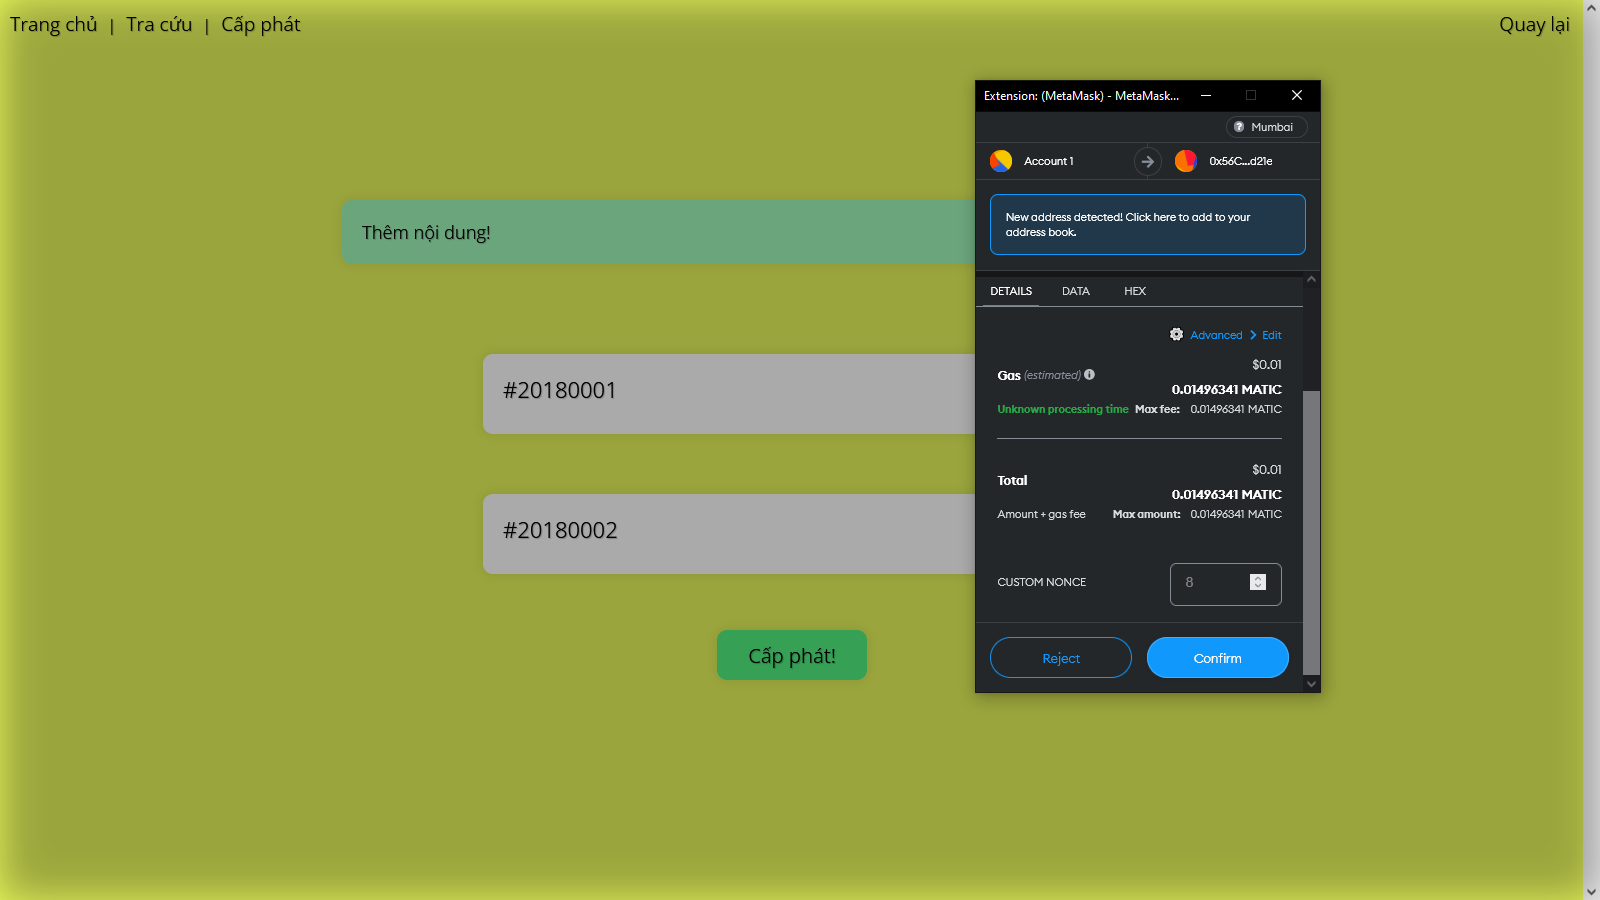
\includegraphics[width=350px]{anh/giai-phap/giao-dien-cap-phat-4.png}
    \caption{Một phần giao diện cấp phát văn bằng (4)}
\end{figure}

\newpage
\begin{figure}[!ht]
    \centering
    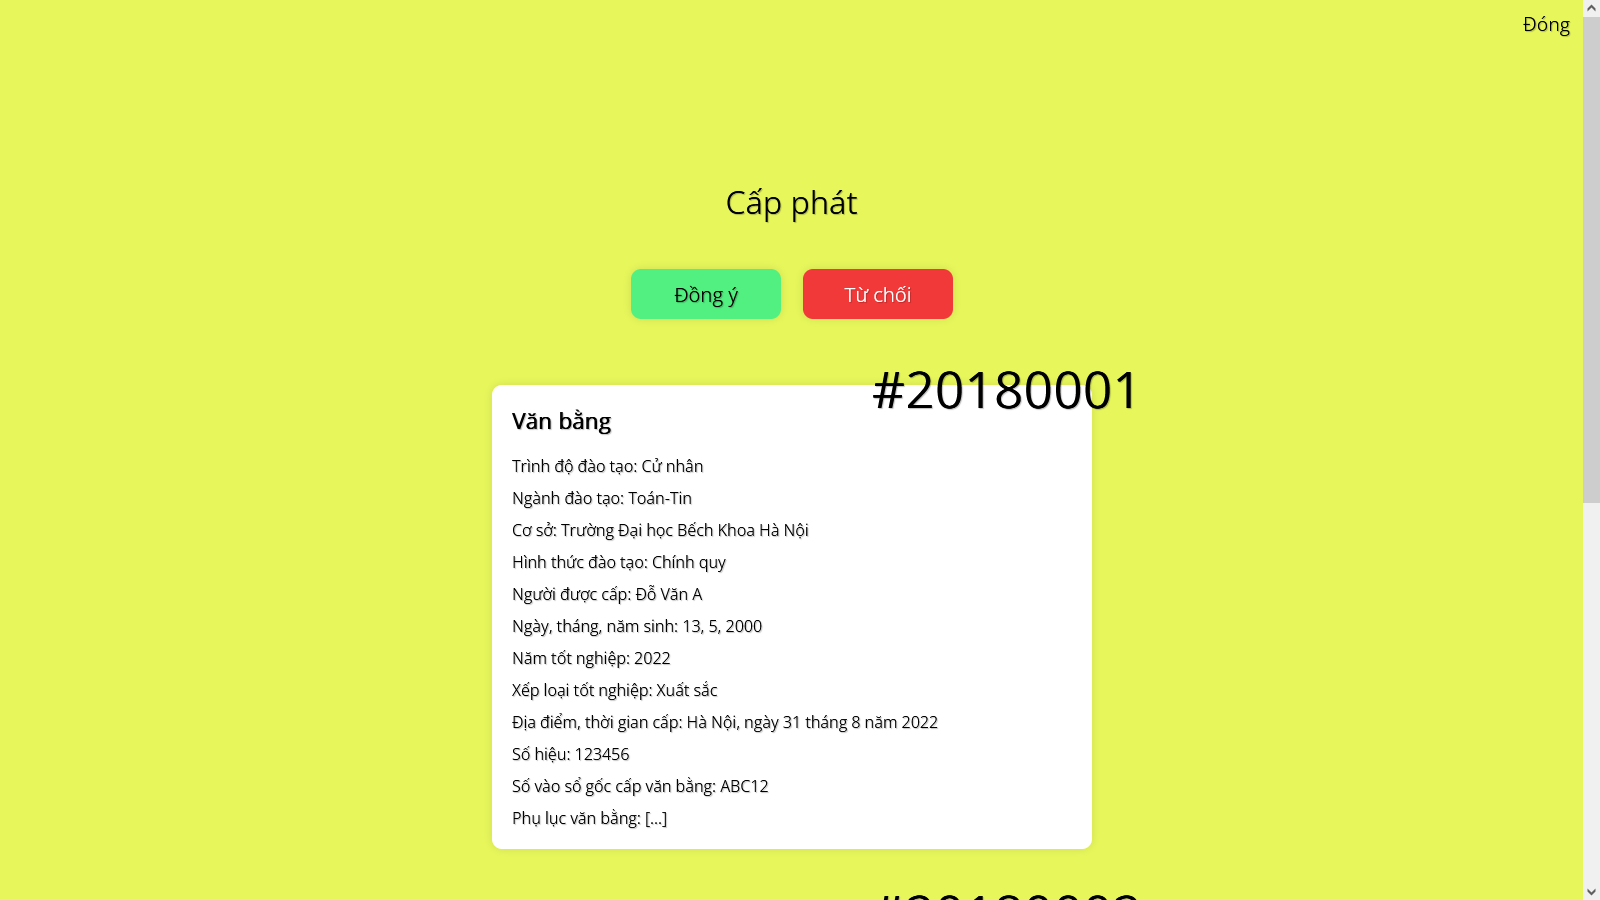
\includegraphics[width=350px]{anh/giai-phap/giao-dien-bau-chon-1.png}
    \caption{Một phần giao diện bầu chọn (1)}
\end{figure}

\begin{figure}[!ht]
    \centering
    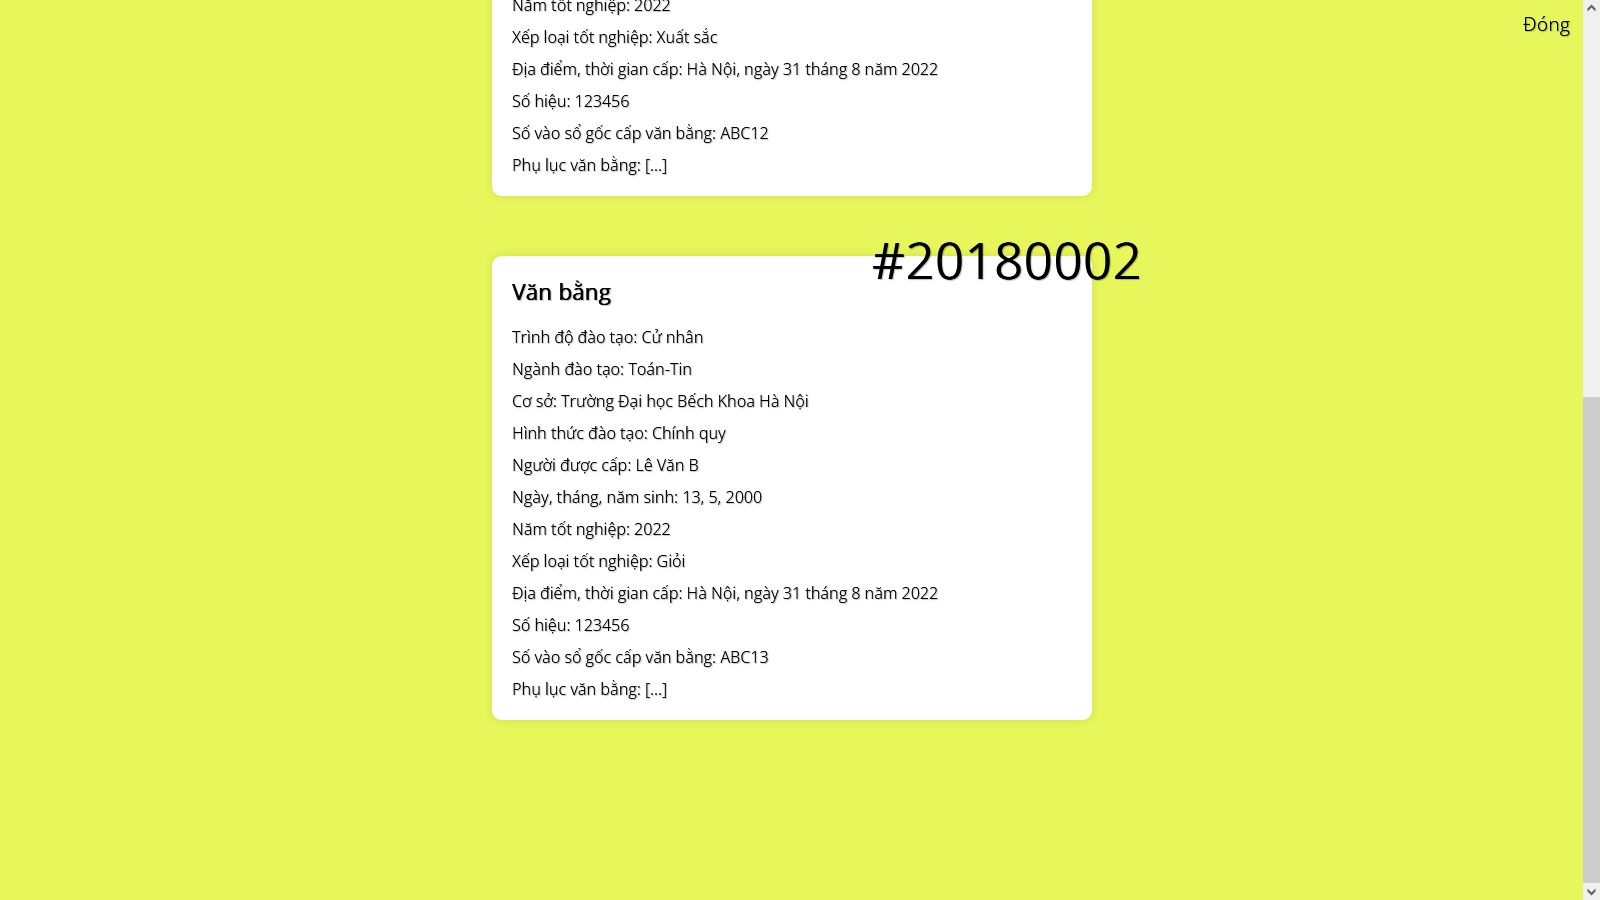
\includegraphics[width=350px]{anh/giai-phap/giao-dien-bau-chon-2.png}
    \caption{Một phần giao diện bầu chọn (2)}
\end{figure}

\newpage
\subsection*{Đánh giá kết quả}

Nhìn chung, các hệ thống ta đã trình bày ở trên đáp ứng tốt các yêu cầu của bài toán đã nêu. Tuy nhiên, một số hạn chế vẫn có thể chỉ ra, như:
\begin{enumerate}
    \item Hiện tại, các hợp đồng thông minh đang được triển khai trên \textit{mạng kiểm thử}\footnote{Testnet} (testnet) nên chi phí giao dịch chưa được đề cập. Nếu triển khai trên \textit{mạng chính}\footnote{Mainnet} của Ethereum, phí giao dịch khá là cao.\label{cons/transaction-fee}
    \item Chưa hỗ trợ đầy đủ các tính năng cần có của một hệ thống cấp phát nội dung (như chỉnh sửa tại trang, thông báo thời gian thực, vân vân), cũng như giao diện chưa được bắt mắt.
\end{enumerate}

Đối với \textit{hạn chế về chi phí giao dịch}, đây là một bài toán khá đau đầu với những \textit{DApp} triển khai trên mạng Ethereum. Tuy nhiên, trong những năm gần đây, rất nhiều giải pháp giảm chi phí và tăng tốc độ xác thực giao dịch trên mạng chuỗi khối đã được đưa ra, trong số đó có thể kể đến như \textit{Plasma}, \textit{Matic}.\\

Các phần bổ sung sẽ được em cân nhắc kỹ lưỡng cho vào thiết kế, phụ thuộc vào mức độ phù hợp với môi trường triển khai thực tế.